% !TeX root = ../../../main.tex

We now repeat the stability and uncertainty
study of the previous section, but for our final
result, namely the intrinsic charm \pdf. The main difference to be kept
in mind is that the uncertainty now also includes the dominant MHOU,
due to the matching condition required in order to determine the 3\fns
\pdf from the 4\fns result. In order to get a complete picture, we now
add a further set of dataset variations.

\paragraph{Dependence on the input dataset.}
%
\cref{fig:ic/charm_dataset_dep_nf3} displays the dataset variations shown in
\cref{fig:ic/charm_dataset_dep}, now for the intrinsic (3\fns) charm
\pdf, but with the total uncertainty now being the sum in quadrature of
the \pdf and MHO uncertainties, with the latter determined as the difference between
results obtained using \nnlo and \nnnlo matching.
%
Additionally, we also performed a few extra  dataset
variations: a fit without any $W, Z$ production data from \atlas and \cms,
a fit without jet data, a fit without $Z$ $p_T$ measurements, and a fit without
HERA structure function data.
%
Note that the collider-only dataset includes both HERA electron-proton
collider data and Tevatron and \lhc hadron collider data, but not
fixed-target deep-inelastic scattering and Drell-Yan production data.


Results are qualitatively very similar to those seen in the 4\fns, a
consequence of the fact that we are focusing on the large-$x$ region where the
effect of the matching is moderate, though now the presence of a
valence-like peak in all determinations is even clearer, specifically
for the DIS-only fit where it was less pronounced in the 4\fns.
%
 Note however that the DIS-only determination
  exhibits larger uncertainties
  (up to factor 2) and point-by-point fluctuations,
  and is dominated by relatively old fixed-target measurements.
%
Comparison of all the dataset variations shows that, in terms of their
impact on intrinsic charm,
hadron collider data are generally more important
that deep-inelastic data, that among the former the
\lhcb inclusive $W,Z$ data are playing a dominant role,
and that jet observables also play a non-negligible role.

It should be stressed that the agreement between results found using
DIS data and hadron collider data is highly nontrivial, since in the region
relevant for intrinsic charm these determinations are based on disjoint datasets
and are  affected by
very different theoretical and experimental uncertainties:
in particular, potential higher-twist
effects in the DIS observables are highly suppressed for collider observables.
%
 this respect, a DIS-only determination of intrinsic charm
  is potentially affected by sources of theory uncertainties, such as higher twists,
which are not accounted for in global \pdf determinations.

%%%%%%%%%%%%%%%%%%%%%%%%%%%%%%%%%%%%%%%%%%%%%%%%%%%%%%%%%%%%%%%%%%%
\begin{figure}[h]
  \begin{center}
    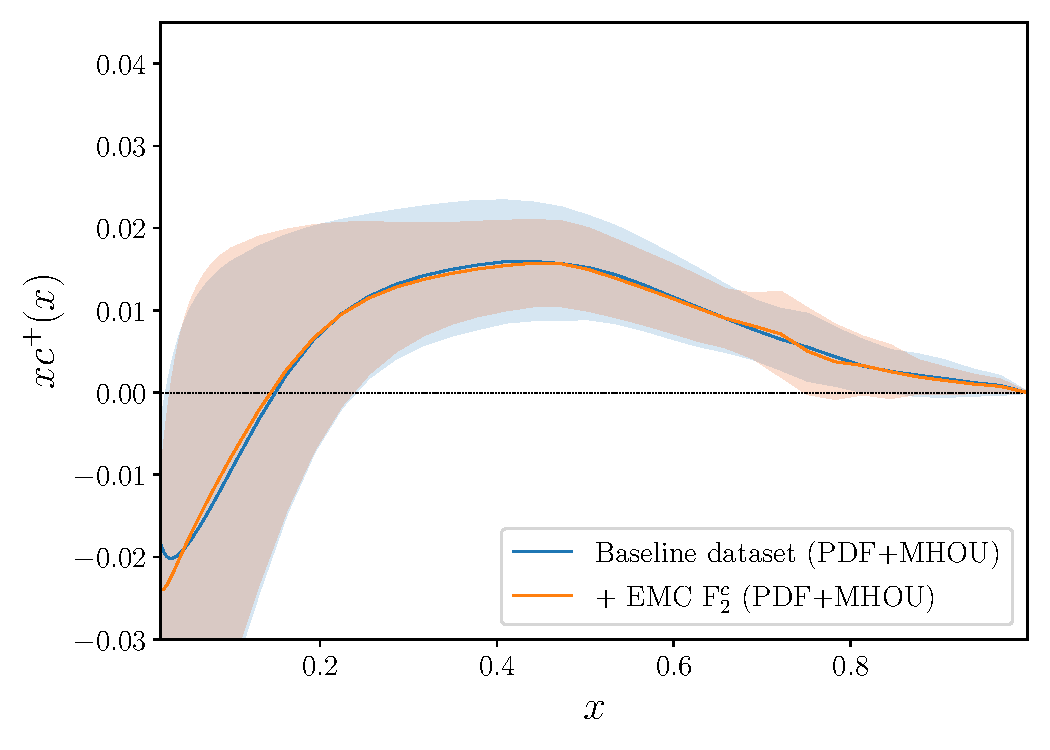
\includegraphics[width=0.49\linewidth]{ch-ic/EMC_Quad_MHOU.pdf}
    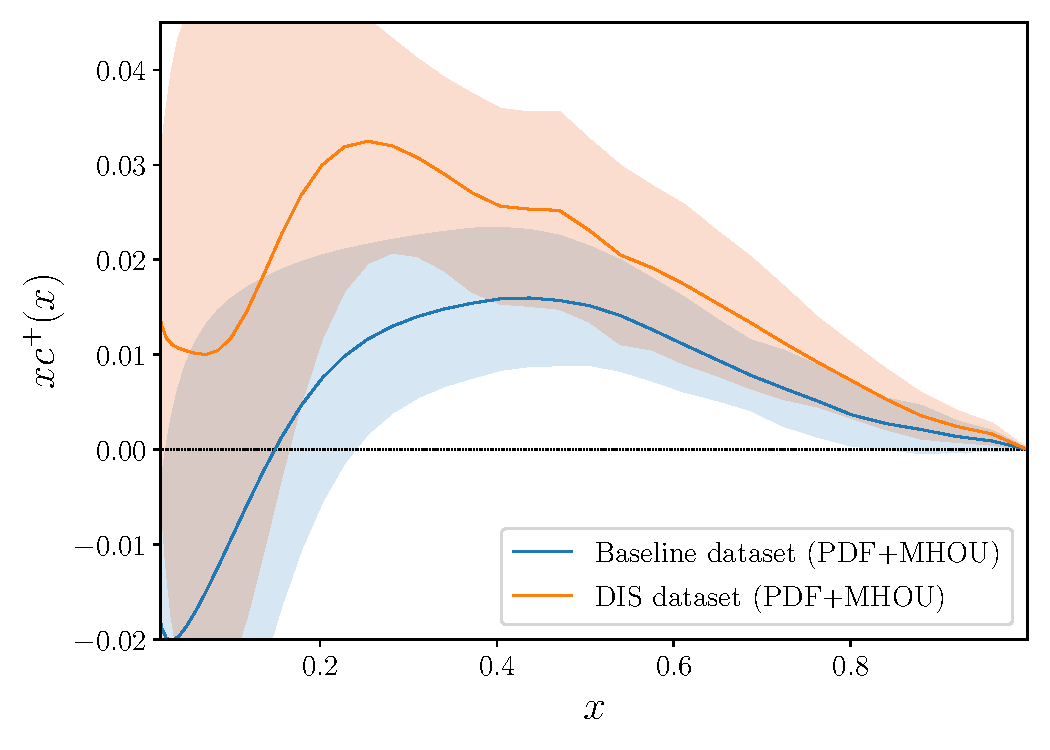
\includegraphics[width=0.49\linewidth]{ch-ic/DIS_only_Quad_MHOU.pdf}
    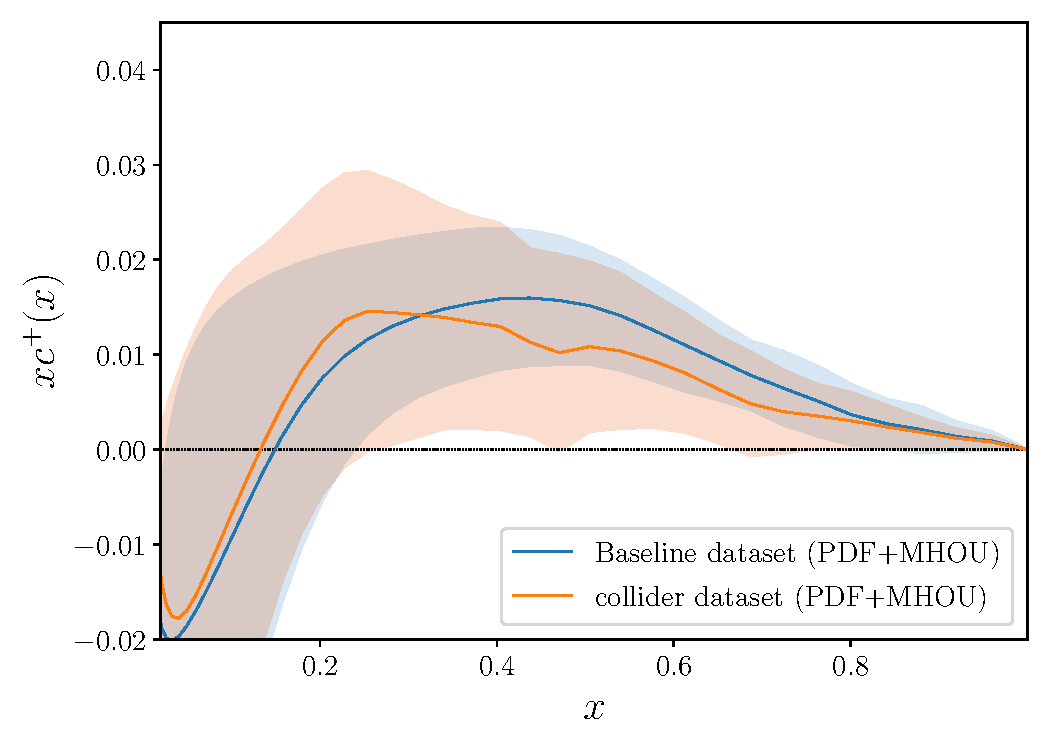
\includegraphics[width=0.49\linewidth]{ch-ic/collider_only_Quad_MHOU.pdf}
    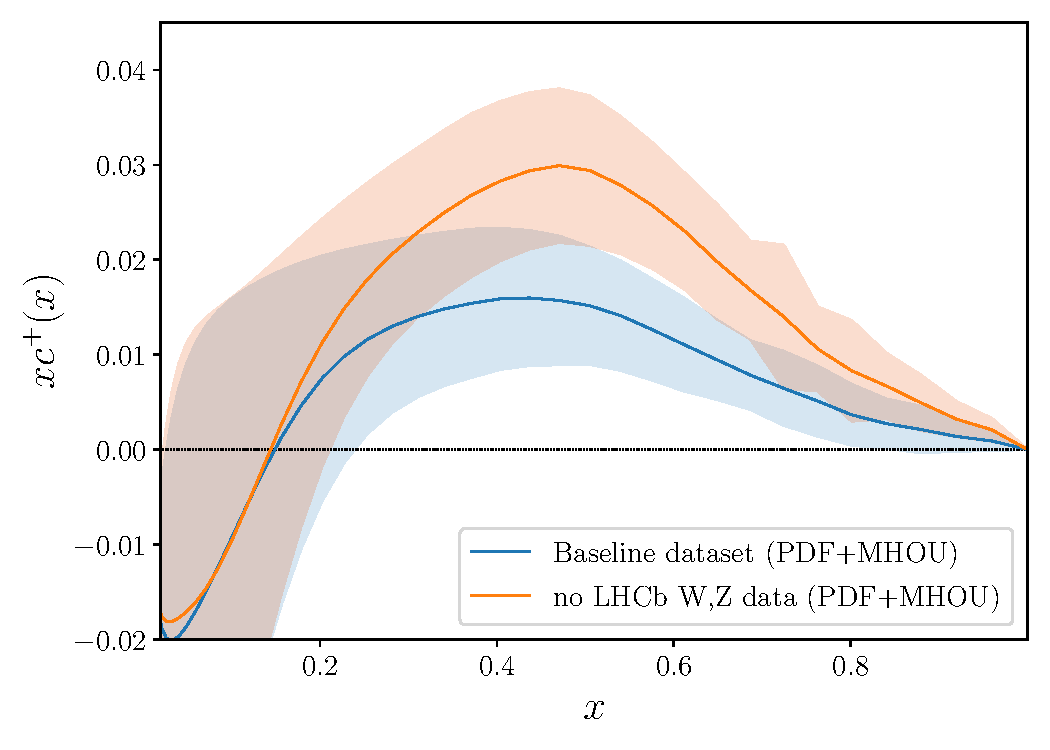
\includegraphics[width=0.49\linewidth]{ch-ic/noLHCb_Quad_MHOU.pdf}
    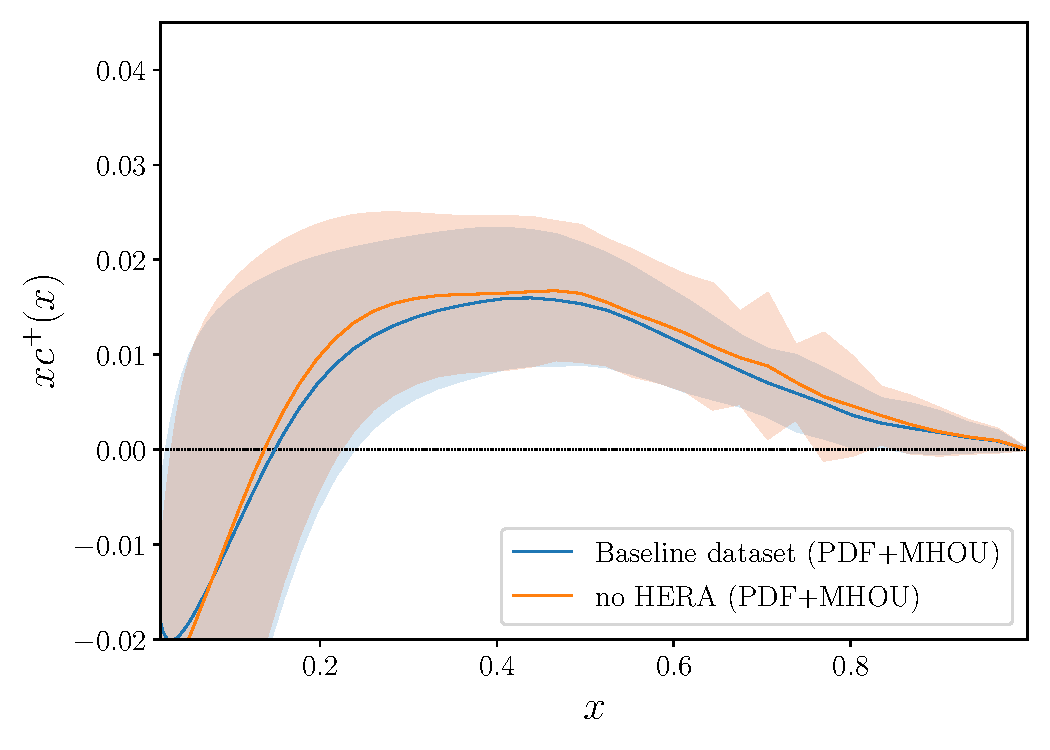
\includegraphics[width=0.49\linewidth]{ch-ic/noHERA_Quad_MHOU.pdf}
    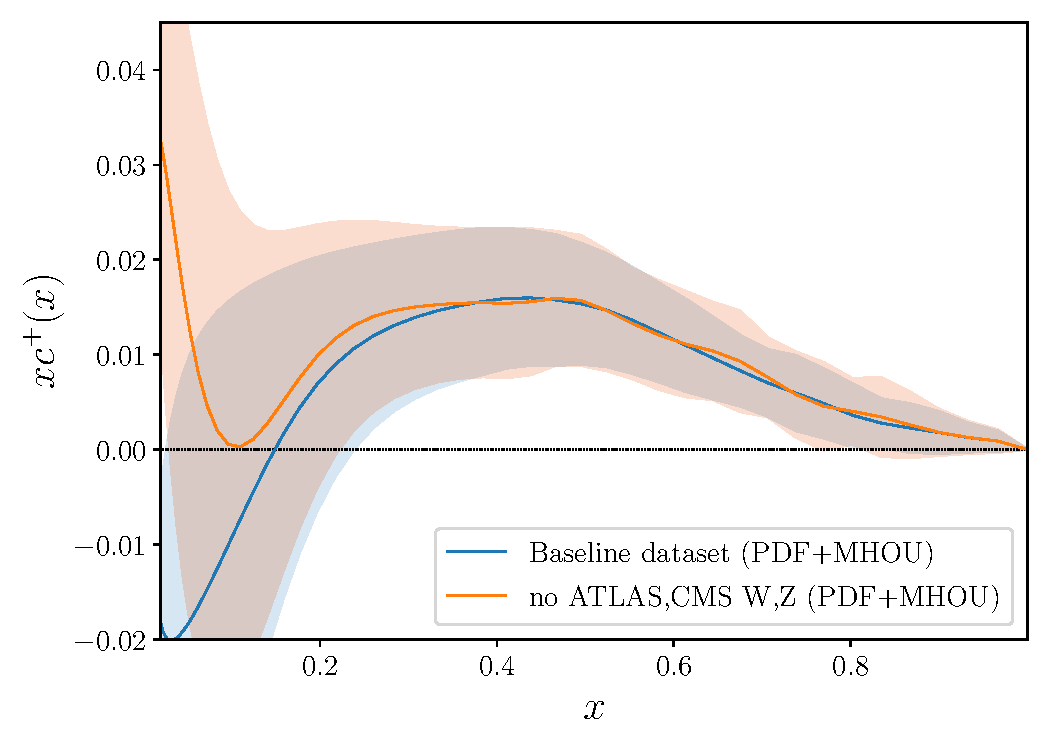
\includegraphics[width=0.49\linewidth]{ch-ic/noATLASCMSDY_Quad_MHOU.pdf}
    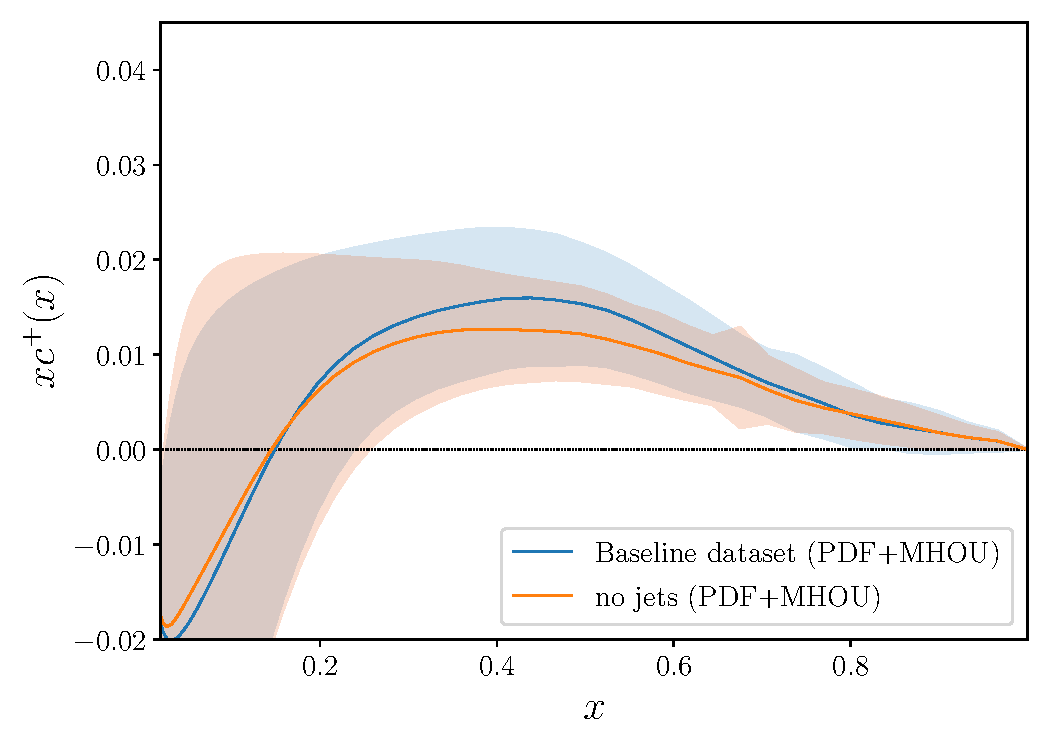
\includegraphics[width=0.49\linewidth]{ch-ic/nojets_Quad_MHOU.pdf}
    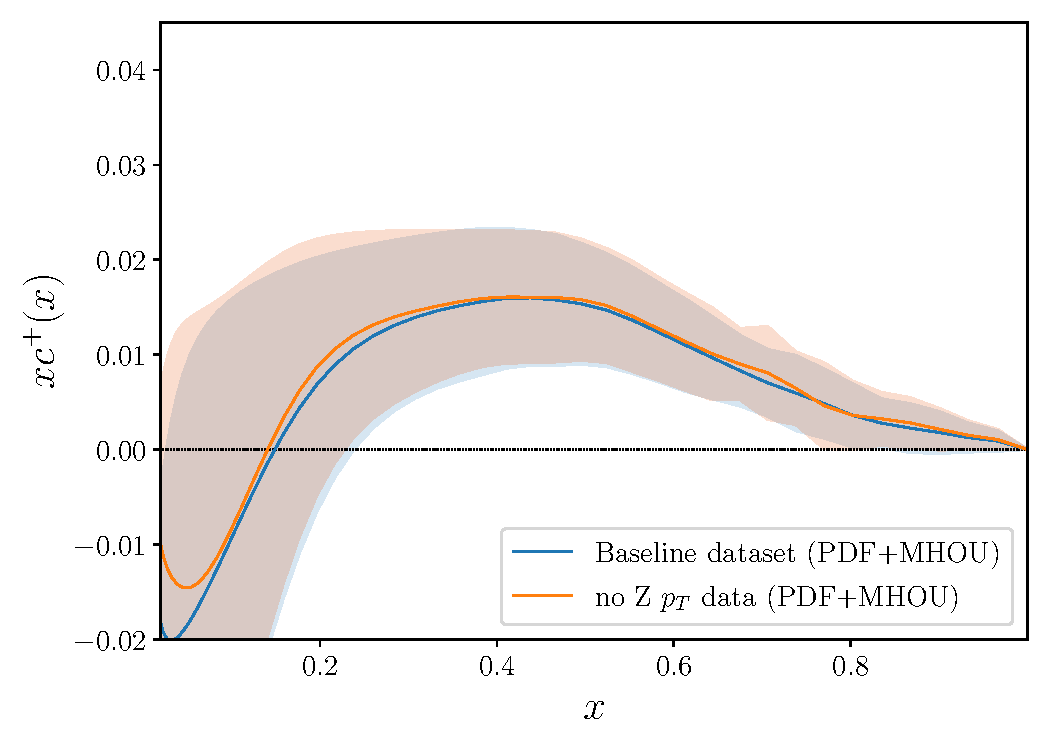
\includegraphics[width=0.49\linewidth]{ch-ic/noZpT_Quad_MHOU.pdf}
    \caption{\small Same as \cref{fig:ic/charm_dataset_dep}
      for the intrinsic charm (3\fns) \pdf (top four plots), now also including
      four additional dataset variations:  no \atlas and \cms $W, Z$
      production data   (third row left),
      no jet data (third row right), no $Z$ $p_T$
      measurements (bottom row left), no HERA
      DIS data (bottom row right).
The error band indicates the \pdf uncertainties combined in quadrature with the MHOUs.
\label{fig:ic/charm_dataset_dep_nf3} }
\end{center}
\end{figure}
%%%%%%%%%%%%%%%%%%%%%%%%%%%%%%%%%%%%%%%%%%%%%%%%%%%%%%%%%%%%%%%%%%%%%%

We conclude that
the characteristic valence-like peak structure at large-$x$
predicted by non-perturbative intrinsic charm models (\cref{fig:ic/charm_content_3fns}
in the main manuscript)
is always present even under very significant changes of the dataset.
%

\paragraph{Dependence on the parametrization basis.}
%
\cref{fig:ic/charm_basisdep_3FNS} displays
the comparison between the intrinsic charm
\pdf determined with the default evolution basis choice, and the flavor
basis. Complete consistency of central values is found, with somewhat
larger uncertainties in the case of the flavor basis, due to the more 
challenging fitting environment in this basis (see the discussion in~\cite{Ball:2021leu}).

%%%%%%%%%%%%%%%%%%%%%%%%%%%%%%%%%%%%%%%%%%%%%%%%%%%%%%%%%%%%%%%%%%%
\begin{figure}[t!]
  \begin{center}
    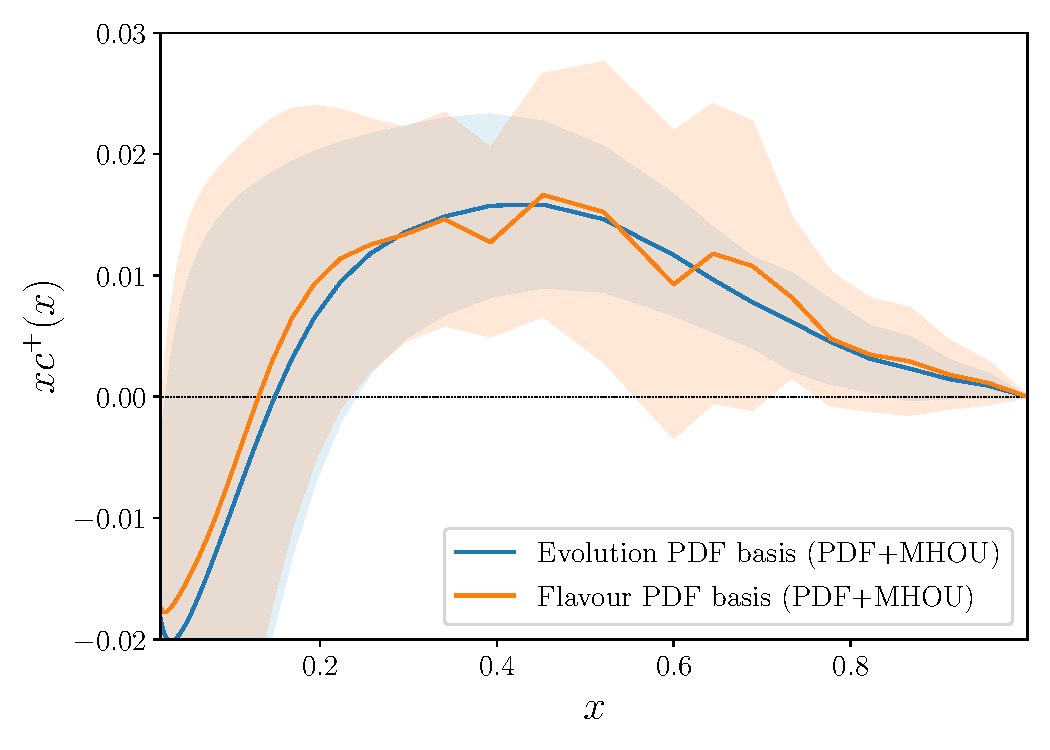
\includegraphics[width=0.54\linewidth]{ch-ic/Flavor_Basis_Quad_MHOU.pdf}
    \caption{\small Same as \cref{fig:ic/charm_basisdep}
    for the intrinsic (3\fns) charm.
  \label{fig:ic/charm_basisdep_3FNS} }
\end{center}
\end{figure}
%%%%%%%%%%%%%%%%%%%%%%%%%%%%%%%%%%%%%%%%%%%%%%%%%%%%%%%%%%%%%%%%%%%%%%


\paragraph{Dependence on the charm mass value.}
%
The study of the charm mass dependence is particularly interesting,
because the intrinsic component should be independent of it, hence the
residual dependence seen in \cref{fig:ic/charm_fitted_mcdep} in the
4\fns, due to the mass dependence of the perturbative component that
could not be reabsorbed in the fitting, should no longer be present. 
Results are shown in
\cref{fig:ic/mass_variations_Quad_MHOU}, and it is apparent that
indeed the dependence on the charm mass has all but disappeared.


%%%%%%%%%%%%%%%%%%%%%%%%%%%%%%%%%%%%%%%%%%%%%%%%%%%%%%%%%%%%%%%%%%%
\begin{figure}[h]
  \begin{center}
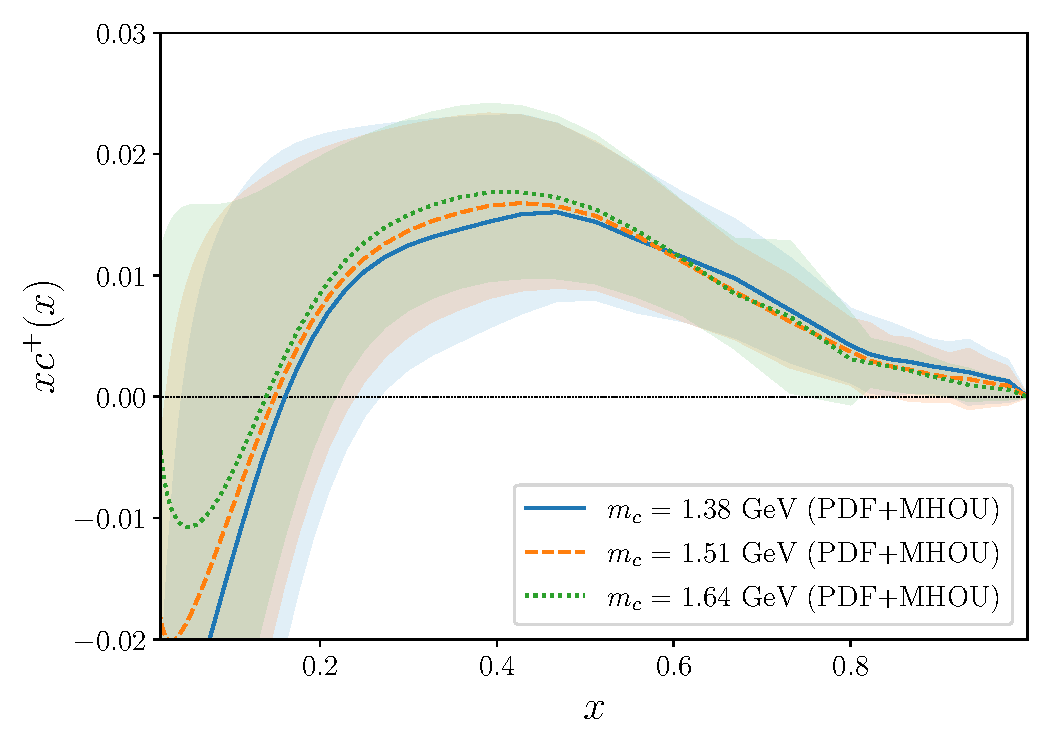
\includegraphics[width=0.49\linewidth]{ch-ic/mass_variations_Quad_MHOU.pdf}
    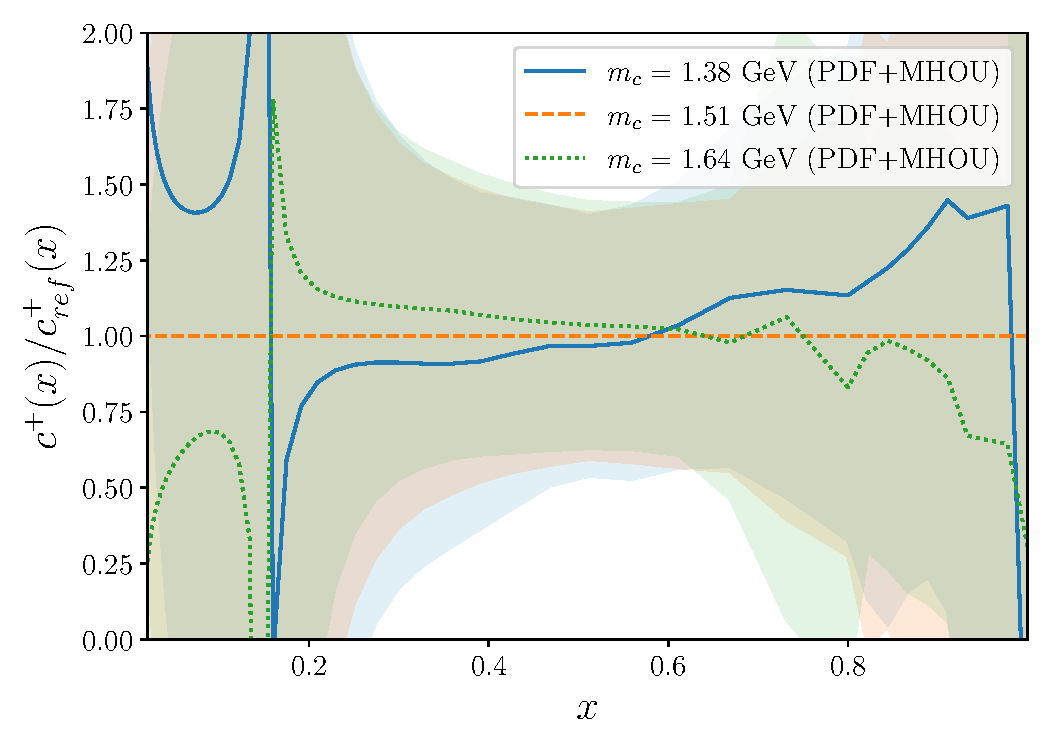
\includegraphics[width=0.49\linewidth]{ch-ic/mass_variations_ratio_Quad_MHOU.pdf}
\caption{\small      
 Same as \cref{fig:ic/charm_fitted_mcdep}, now for
      the intrinsic (3\fns) charm \pdf. Note that the intrinsic charm
      \pdf is scale independent.
  \label{fig:ic/mass_variations_Quad_MHOU} }
\end{center}
\end{figure}
%%%%%%%%%%%%%%%%%%%%%%%%%%%%%%%%%%%%%%%%%%%%%%%%%%%%%%%%%%%%%%%%%%%%%%
